\documentclass[../en-fa-lab.tex]{subfiles}


\usepackage{hyperref}

\hypersetup{
    pdftitle={(EN) L6 - Multi-way trees},   % The title shown in the browser tab
    pdfauthor={},         % Your name or organization
    pdfsubject={},   % A brief description
    pdfkeywords={}
}

\begin{document}

\section{\texorpdfstring{\textbf{Assignment No. 6: Multi-way Trees }}{Assignment No. 6: Multi-way Trees}}\label{assign6}

\emph{\textbf{Transforms between different representations}}
\textbf{Allocated time:} 2 hours

\subsection{Implementation}\label{implementation}

\begin{enumerate}
\def\labelenumi{\arabic{enumi}.}
\item
  You are required to implement \textbf{correctly} and
  \textbf{efficiently} \emph{iterative} and \emph{recursive} binary tree
  traversal. You may find any necessary information and pseudo-code in
  your course and seminar notes.
\item
  Moreover, the \textbf{correct} and \textbf{efficient} implementation
  of \emph{linear} complexity algorithms is required for transforming
  multi-way trees between the following representations:

  \begin{enumerate}
  \def\labelenumii{\arabic{enumii}.}
  \item
    \textbf{R1}: \emph{Parent representation}: for each index, the value
    in the vector represents the parent\textquotesingle s index, e.g.:
    \(\Pi = \{ 2,7,5,2,7,7, - 1,5,2\}\)
  \item
    \textbf{R2}: \emph{Multi-way tree representation}: each node
    contains the key and a vector of child nodes.
  \item
    \textbf{R3}: \emph{Binary representation}: each node contains the
    key and two pointers, one to the first child and the second to the
    right sibling (e.g., the next sibling).
  \end{enumerate}
\end{enumerate}

Therefore, you need to define transformation \textbf{T1} from the
\emph{parent representation} (\textbf{R1)} to the \emph{multi-way tree
representation} (\textbf{R2}), and then the transformation \textbf{T2}
from the \emph{multi-way tree representation} (\textbf{R2}) to the
\emph{binary representation} (\textbf{R3}). For all representations
(\textbf{R1}, \textbf{R2}, \textbf{R3}), you need to implement the
Pretty Print (\textbf{PP}) display (see page 2).

Define the data structures. You can use intermediate structures (e.g.,
additional memory).

\subsection{Requirements}\label{requirements}

\subsubsection{\texorpdfstring{Implementation of \emph{iterative} and
\emph{recursive} binary tree traversal in \emph{O(n)} and \emph{with
constant additional memory}
(3p)}{Implementation of iterative and recursive binary tree traversal in O(n) and with constant additional memory (3p)}}\label{implementation-of-iterative-and-recursive-binary-tree-traversal-in-on-and-with-constant-additional-memory-3p}

You will have to prove your algorithm(s) work on a small-sized input.

\subsubsection{Implementation of transforms between different
representations}\label{implementation-of-transforms-between-different-representations}

\subsubsection{Correct implementation for Pretty-print for R1
(2p)}\label{correct-implementation-for-pretty-print-for-r1-2p}

\subsubsection{\texorpdfstring{Correct implementation for \emph{T1 (from R1
to R2)} and pretty-print for \emph{R2} (1p) + \emph{T1} in linear time
(1p)}{Correct implementation for T1 (from R1 to R2) and pretty-print for R2 (1p) + T1 in linear time (1p)}}\label{correct-implementation-for-t1-from-r1-to-r2-and-pretty-print-for-r2-1p-t1-in-linear-time-1p}

\subsubsection{\texorpdfstring{Correct implementation for \emph{T2}
\emph{(from R2 to R3)} and pretty-print for \emph{R3} (2p) + \emph{T2}
in linear time
(1p)}{Correct implementation for T2 (from R2 to R3) and pretty-print for R3 (2p) + T2 in linear time (1p)}}\label{correct-implementation-for-t2-from-r2-to-r3-and-pretty-print-for-r3-2p-t2-in-linear-time-1p}

The correctness of the algorithms should be demonstrated using the
example \(\Pi = \{ 2,7,5,2,7,7, - 1,5,2\}\).

Use Pretty Print for all three representations. \emph{Each
representation (R1,R2,R3) should have a pretty print of its own with a
different implementation but with the same print.}

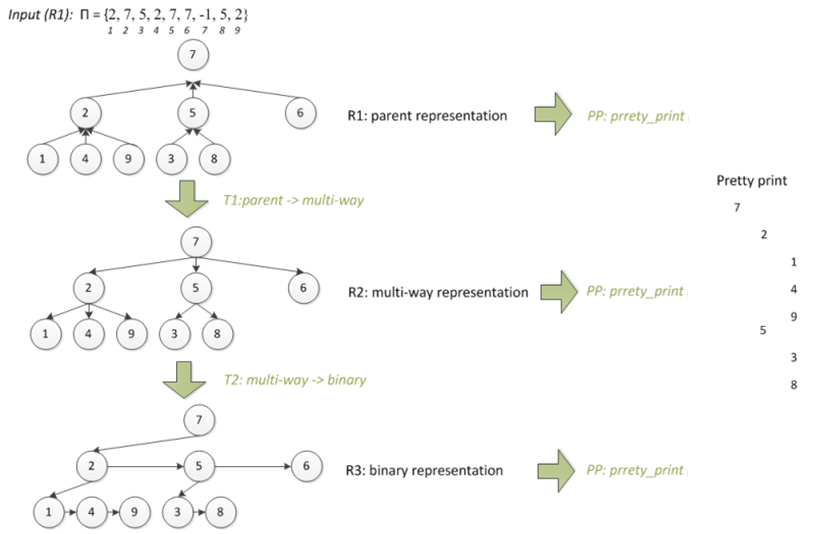
\includegraphics[width=\textwidth]{../Resources/lab6/Lab6_representations.png}

Analyse the time and space efficiency of the two transformations. Did
you achieve \emph{O(n)}? Did you use additional memory?

\end{document}